\chapter{Лабораторная работа №7 \\
\Large Определение модуля упругости первого рода материалов методом колебаний}

Цель работы: ознакомление с методикой и аппаратурой и определение модуля упругости первого рода различных материалов.

Оборудование и инструменты: вибростенд (генератор, усилитель, вибростол), микрометр, штангенциркуль.

\section{Теоретическая часть}

Упругостью называют свойство материала девормироваться под действием нагрузки и восстанавливать свою первоначальную форму после разгрузки.

Согласно закону Гука напряжение и вызванная им деформация связаны между собой прямо пропорциональной зависимостью.
При одноосном напряжённом состоянии закон Гука выражается формулой
\[
    \sigma = \epsilon E.
\]

Закон Гука соблюдается только на начальной стадии нагружения, пока напряжение не превышает предела пропорциональности материала.

В настоящей лабораторной работе определение модуля упругости первого рода $E$ основано на анализе связи его с частотой поперечных резонансных колебаний консольно закреплённой пластинки постоянного сечения $F = bh$, длиной $l$ (рис. \ref{fig:force-scheme}).

\begin{figure}[!ht]
    \centering
    \includegraphics[width=0.7\textwidth]{force-scheme}
    \caption{Силовая рассчётная схема}
    \label{fig:force-scheme}
\end{figure}

Участок пластинки длиной $dz$ имеет массу $dm = \rho F dz$, где $\rho$ "--- плотность материала.

Инерционная сила, приходящаяся на единицу длины пластинки при поперечном перемещении $y$, запишется как $q = -\rho F \ddot{y}$, где $F$ "--- площадь сечения пластинки.
Знак <<минус>> означает, что нагрузка $q$ направлени в сторону, противоположную прогибу.
% Из теории изгиба известно, что 

Дифференциальное уравнение поперечных колебаний пластинки имеет вид
\begin{equation}\label{eq:partial-equation}
    \frac{\partial^4 y}{\partial z^4} + \frac{\rho F}{E I} \frac{\partial^4 y}{\partial z^4} = 0,
\end{equation}
где $I$ "--- момент инерции; $t$ "--- время.

Решение уравнения \eqref{eq:partial-equation} можно представить в виде $y = Z \sin \omega$, где $\omega$ "--- угловая частота.
После подстановки его в \eqref{eq:partial-equation} получим
\begin{align}
    Z^{(IV)} - \alpha z = 0, \label{eq:diff-equation} \\
    \alpha^4 = \frac{\rho F \omega^2}{E I}. \label{eq:alpha-equation}
\end{align}
    
Решение уравнения (\ref{eq:diff-equation}) запишем в общем виде:
\begin{equation}\label{eq:general-solve}
    Z = A \sin(\alpha z) + B \cos(\alpha z) + C \sh(\alpha z) + D \ch(\alpha z),
\end{equation}
где $А$, $В$, $С$, $D$ "--- постоянные, которые определяются из граничных условий.

Для консольно закрепленной балки функция (\ref{eq:diff-equation}) имеет следующие граничные условия: при $z = 0$ $Z = 0$ и $\frac{dZ}{dz} = 0$, на конце балки (при $z = l$) изгибающий момент и поперечная сила равны нулю.
Следовательно, при $z = l$, $\frac{d^2z}{dz^2} = 0$ и $\frac{d^3z}{dz^3}= 0$.

Составим определитель этой системы и приравняем его нулю:
\[
    \left|\begin{array}{cccc}
        0 & 1 & 0 & 1 \\
        1 & 0 & 1 & 0 \\
        -\sin (\alpha l) & \cos (\alpha l) & \sh (\alpha l) & \ch (\alpha l) \\
        -\cos (\alpha l) & \sin (\alpha l) & \ch (\alpha l) & \sh (\alpha l)
    \end{array}\right|
    = 0,
\]

Подставляя граничные условия в (\ref{eq:general-solve}), имеем четыре уравнения:
\begin{equation}
    \begin{cases}
        A + D = 0 \\
        A + C = 0 \\
        -A \sin (\alpha l) - B \cos (\alpha l) + C \sh (\alpha l) + D \ch (\alpha l) = 0 \\
        -A \cos (\alpha l) + B \sin (\alpha l) + C \ch (\alpha l) + D \sh (\alpha l) = 0
    \end{cases}
\end{equation}
откуда следует $\ch (\alpha l) \cdot \cos (\alpha l) = -l$.
Последовательный ряд корней этого уравнения имеет вид $\alpha_1 l = 1.875$, $\alpha_2 l = 4.694$, $\alpha_3 l = 7.855$ и т.д.

\begin{figure}[!ht]
    \centering
    \begin{subfigure}[t]{0.5\textwidth}
        \centering
        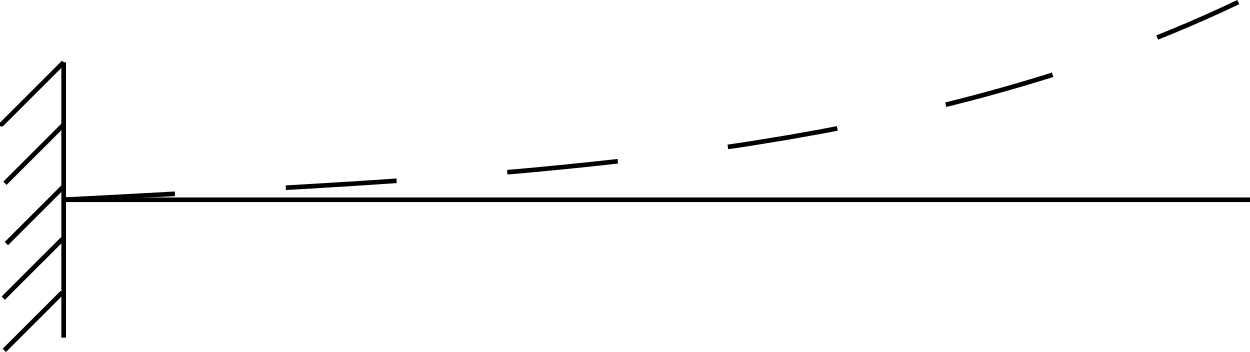
\includegraphics[width=\textwidth]{resilient-line-form-1}
        \caption{}
    \end{subfigure}
    \begin{subfigure}[t]{0.5\textwidth}
        \centering
        \includegraphics[width=\textwidth]{resilient-line-form-2}
        \caption{}
    \end{subfigure}
    \begin{subfigure}[t]{0.5\textwidth}
        \centering
        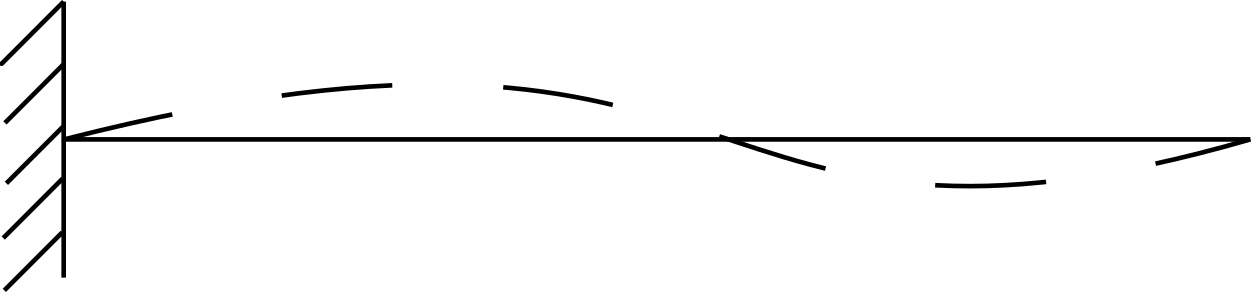
\includegraphics[width=\textwidth]{resilient-line-form-3}
        \caption{}
    \end{subfigure}
    \caption{Форма упругой линии балки при достижении резонанса: а) на первой собственной частоте; б) на второй; в) на третьей.}
    \label{fig:resilient-line-form}
\end{figure}

Первые три формы изгиба пластинки, соответствующие трём корням уравнения, изображены на рис. \ref{fig:resilient-line-form}.
Эти формы можно наблюдать в моменты резонанса, увеличивая частоту колебаний вибростола с консольно закрепленной пластинкой.

Выражение \eqref{eq:alpha-equation}, разрешённое относительно модуля упругости, запишется в виде
\[
    E = \frac{\rho F}{I_x} \omega^2 \frac{I^4}{(\alpha l)^4}.
\]

С учетом $F = b h$, $I_x = \frac{b h^3}{12}$, $\omega = 2 \pi f$ получаем:
\[
    E = \frac{12 \rho}{h^2} 4 \pi^2 f^2 \frac{l^4}{(\alpha l)^4},
\]
где $f$ "--- частота резонансных колебаний в Герцах.

Таким образом, по полученной форме колебаний можно вычислить модуль упругости первого рода $E$, фиксируя резонансную частоту и подставляя соответствующее значение $al$.

Для первой формы ($al = 1.875$):
\begin{equation}\label{eq:resilience-module-1}
    E = \frac{48 \rho}{h^2} \pi^2 f_1^2 \frac{l^4}{1.875^4};
\end{equation}

Для второй формы ($al = 4.694$):
\begin{equation}\label{eq:resilience-module-2}
    E = \frac{48 \rho}{h^2} \pi^2 f_1^2 \frac{l^4}{1.875^4};
\end{equation}

Для третьей формы ($al = 7.855$):
\begin{equation}\label{eq:resilience-module-3}
    E = \frac{48 \rho}{h^2} \pi^2 f_1^2 \frac{l^4}{1.875^4};
\end{equation}

\section{Лабораторный стенд}
Для экспериментального определения собственной частоты пластинки в настоящей работе использован вибростенд, схема которого приведена на рис. \ref{fig:vibration-testbench}.

\begin{figure}[!ht]
    \centering
    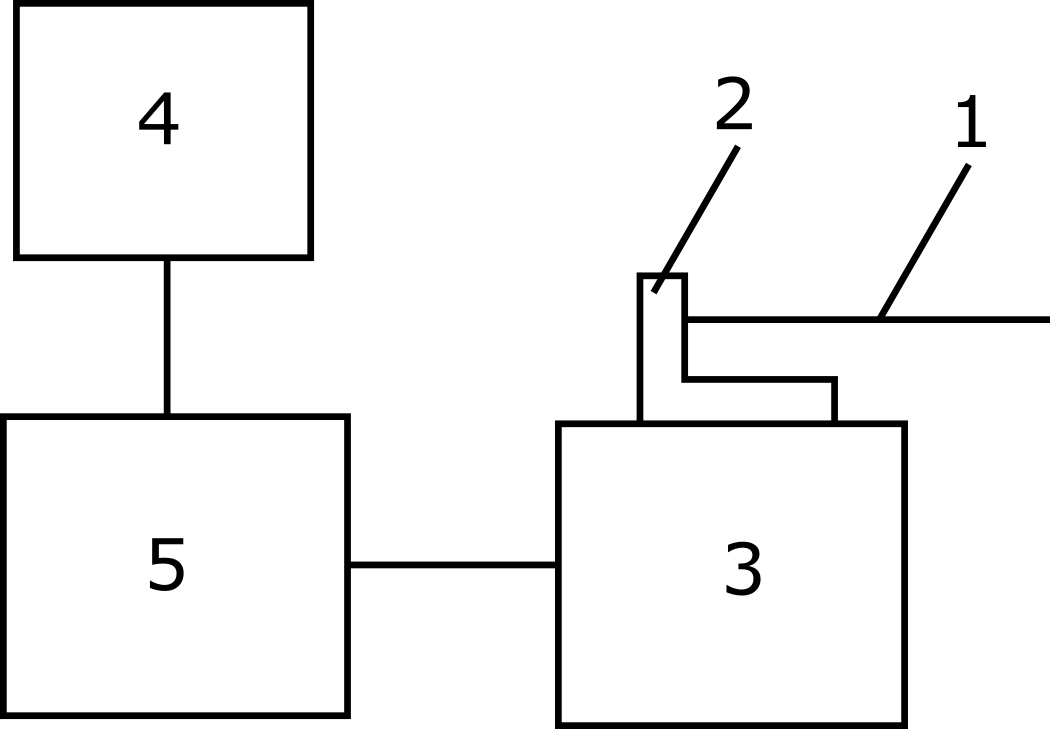
\includegraphics[width=0.6\textwidth]{vibration-testbench}
    \caption{Схема вибростенда: 1 "--- испытуемая пластина, 2 "--- зажимное приспособление, 3 "--- вибростол, 4 "--- генератор стандартных сигналов, 5 "--- усилитель}
    \label{fig:vibration-testbench}
\end{figure}

Испытуемая пластинка 1 консольно закреплена в приспособлении 2 на поверхности вибростола 3.
Колебания изменяемой частоты задаются генератором стандартных сигналов 4, амплитуда которых увеличивается усилителем 5.

Частоту колебаний стола можно изменять генератором от нуля до $12 ~кГц$, а уровень амплитуды сигнала регулировать как генератором, так и усилителем.

\section{Практическая часть}
1. Измерим размеры испытуемых пластинок $b$, $h$ микрометром и после закрепления на вибростоле измерим длину $l$ штангенциркулем.
Результаты занесём в таблицу (табл. \ref{tab:results}).

\begin{table}[H]
    \centering
    \caption{Результаты измерений и вычислений}
    \label{tab:results}
    \begin{tabular}{|l|c|c|c|c|}
        \hline
        \multirow{2}{*}{Параметры пластины}               & \multicolumn{4}{c|}{Материал пластинки} \\ \cline{2-5}
                                                          & 29НК & Медь М-1 & Кремний & Керамика \\ \hline
        Толщина $h, мм$                                   & 0.21 & 0.31 & 0.35  & 0.82 \\ \hline
        Плотность $\rho, 10^{-9}~\frac{Н \cdot с^2}{мм^4} $ & 8.35 & 8.96 & 2.33  & 3.60 \\ \hline
        Длина $l, мм$                                     & 73.1 & 74.5 & 63.0  & 75.7 \\ \hline
        Резонансная частота $f_1, Гц$                     & 27.5 & 30.0 & 116.0 & 172  \\ \hline
        Резонансная частота $f_2, Гц$                     & 171  & 184  & -     & -    \\ \hline
        Модуль $E', МПа$                                  & 1.57 & 0.99 & 1.55  & 1.99 \\ \hline
        Модуль $E'', МПа$                                 & 1.54 & 0.95 & -     & -    \\ \hline
    \end{tabular}
\end{table}

2. Плавно изменяя частоту задающего генератора, зафиксируем резонансную частоту $f_1$.
Увеличивая частоту, зафиксируем резонансную частоту $f_2$.

3. Изменим длину консоли пластинки $l$ и повторим измерения резонансных частот $f_1$, $f_2$ при новой длине $l_i$.

4. Вычислим модуль упругости $E$ для кажной резонансной чпстоты и каждой длины консоли закрепления по формулам \eqref{eq:resilience-module-1}\==\eqref{eq:resilience-module-3}.

Вывод: в результате проведённого эксперимента определили упругую характеристику материалов электронной техники.
Метод наглядный, универсальный, не требует разрушения образца.

Недостаток стенда состоит в том, что резонансная частота определяется визуально.

Полученные значения модуля упругости $E$ близки к табличным.

